% ============================================================
% Chapter 2: Background and Literature Review
% ============================================================
\chapter{Background and Literature Review}
\label{chap:background_lit_review}

This chapter provides the necessary technical and historical context for the research presented. It begins by detailing the specific prior work that forms the foundation of this project, illustrated with block diagrams (\Cref{fig:block_diagram_comparison,fig:ayoub_test_setup}), and outlines the practical hardware challenges encountered at the project's outset (\Cref{sec:specific_background}). Subsequently, it reviews the broader context of reverse engineering and obsolescence management in safety-critical systems (\Cref{sec:re_obsolescence}), relevant railway industry retrofitting practices (\Cref{sec:industry_practices}), the applicable functional safety standards framework (\Cref{sec:standards_detail}), and pertinent electronic design principles~\cite{jones2004} (\Cref{sec:design_principles}) that informed the hardware implementation.

% ------------------------------------------------------------
\section{Specific Project Background and Challenges}
\label{sec:specific_background}

This research directly builds upon efforts initiated in previous projects to modernise a specific legacy anti-skid system~\cite{rexroth1992wsp} used in European public transport. Understanding this lineage, the technical foundations laid, and the inherited challenges is necessary for contextualising the methodology and results presented herein.

\subsection{Foundational Reverse Engineering (Ayoub)}
\label{subsec:ayoub_vorarbeit}

The initiative commenced with foundational reverse engineering by Samy Ayoub in 2014~\cite{ayoub2014}, driven by the obsolescence of the processor on the system's comparator (V-) card, which was no longer available. Ayoub's work focused on the feasibility of replacing this processor by emulating its function within an~\gls{fpga}.

Ayoub analysed the original schematic and board, read out and disassembled the program memory (about \SI{2}{\kilo\byte} of assembler code) and decided to keep the program unchanged and to run it on a~\gls{cpu} emulated in an~\gls{fpga}; the emulated~\gls{cpu} was taken over from an earlier project~\cite{ayoub2014}. He verified the design with functional and timing testbenches in~\gls{vhdl} simulation, loaded the individual designs onto~\gls{fpga} boards to test them under real conditions, and compared the rebuilt timer directly with the original one using a microcontroller-based test system~\cite{ayoub2014}. The architecture of the original card is shown in~\Cref{fig:block_diagram_comparison}~(top), his redesign at the bottom.

Ayoub also designed a test setup for comparing the new card with the original (\Cref{fig:ayoub_test_setup}). When he reported, the fully populated card was in its basic function test, the test board was waiting for components, and layout errors had made a new revision of the card necessary~\cite{ayoub2014}. His work outlined a pathway to modernisation that preserves the existing, field-tested control program, thereby reducing the effort and risk associated with developing entirely new control logic, and subsequent work built on it.

\begin{figure}[htbp]
	\centering
	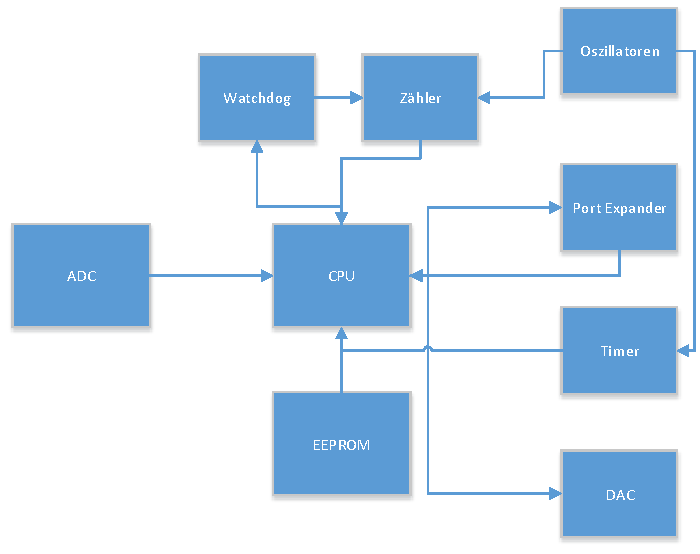
\includegraphics[scale=0.85]{ayoub/comparator_card_original.pdf}\\[3ex]
	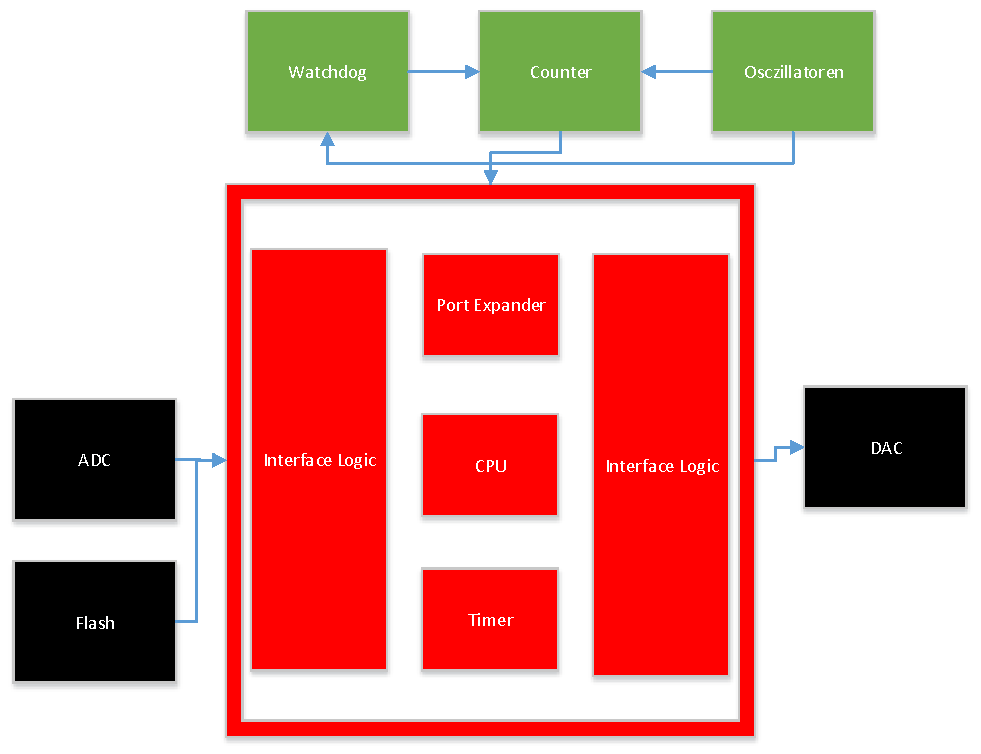
\includegraphics[scale=0.85]{ayoub/comparator_card_fpga.pdf}
	\caption[Block Diagrams of the Comparator Card]{Conceptual block diagrams of the comparator card: the original (top) and Ayoub's \gls{fpga}-based redesign (bottom), in which the red frame encloses the content of the \gls{fpga}, black elements are new and green ones were taken over from the original card. Reproduced as vector graphics from~\cite[Figs.~1 and~3]{ayoub2014}; the German labels are those of the original.}
	\label{fig:block_diagram_comparison}
\end{figure}

% the test setup is wide and its labels are small: it goes on a landscape page
\afterpage{%
\begin{landscape}
\begin{figure}[htbp]
	\centering
	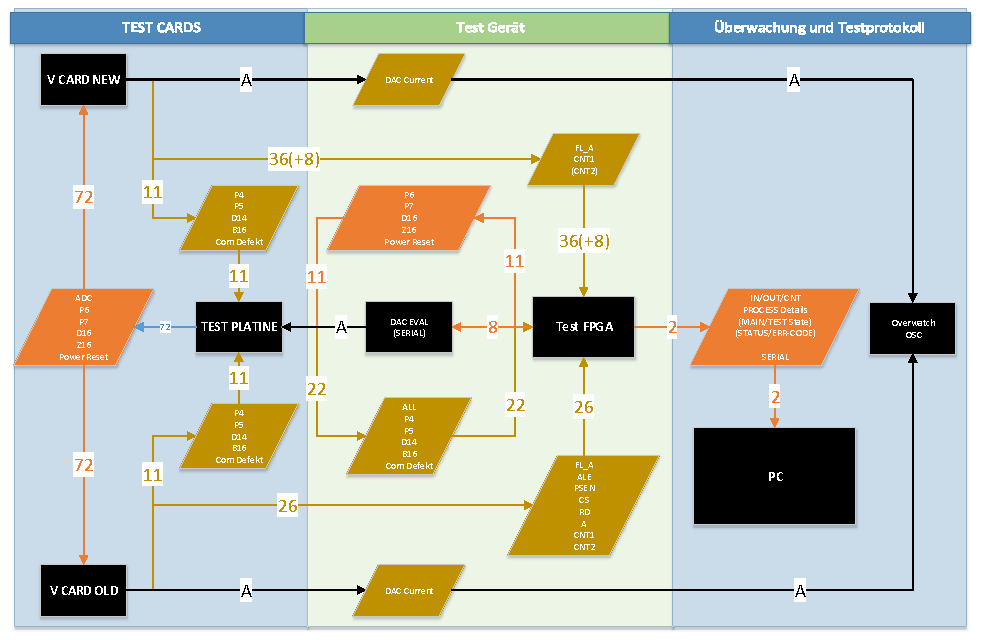
\includegraphics[height=0.82\textheight]{ayoub/test_setup.pdf}
	\caption[Ayoub Test Setup Concept]{Conceptual test setup for verifying the comparator card (German: \foreignlanguage{ngerman}{\textit{Vergleicherkarte}}) against the original, as documented in the preliminary work~\cite{ayoub2014}. Reproduced as a vector graphic from~\cite[Fig.~7]{ayoub2014}; the German labels are those of the original, and the three column headings are raster images in the original.}
	\label{fig:ayoub_test_setup}
\end{figure}
\end{landscape}}

\subsection{Test-Diagnosis Board Retrofit Attempt (Leyer)}
\label{subsec:leyer_internship}

Building on Ayoub's findings, Mark Leyer's 2023 internship project applied the~\gls{fpga} emulation strategy to the legacy system's test-diagnosis board~\cite{leyer2023}. This board, based on the 8035~\cite{leyer2023ppt}, the version of the 8048 without internal program memory~\cite[p.~1-2]{intel_mcs48_1978}, performs non-real-time diagnostics and self-test functions, including fault code storage and retrieval via a 7-segment display and initiation of a system self-test with frequency sweep output.

Leyer migrated the processor and its peripheral functions, namely the frequency sweep, the display driving, the button handling and the interface to the~\gls{nvram}, into~\gls{hdl} targeting an Actel ProASIC3 \texttt{A3P1000}~\gls{fpga}~\cite[Fig.~2]{leyer2023}, whose flash-based configuration memory is non-volatile, in contrast to alternatives based on~\gls{sram}.

Recognising the limitations of the legacy system's simple numeric code feedback, Leyer also designed an auxiliary diagnostics subsystem on a separate~\gls{pcb}~\cite{leyer2023, leyer2023ppt}. Centred on an~\gls{stm32} microcontroller (\texttt{STM32F401RET6}, \Cref{fig:schematic_sheet4}), the board was to provide modern data logging: errors timestamped via~\gls{rtc}, persistent storage on an~\gls{sd}~card and access over~\gls{usb}. A key design principle, critical for functional safety, was maintaining physical and electrical isolation between this non-safety-related logging function and the core safety-related~\gls{fpga} emulation, through an optocoupled~\gls{spi} link (\Cref{sec:stm32_details}).

While a single final test by Leyer showed the prototype behaving like the original system at start-up~\cite[Sec.~9.1]{leyer2023}, the prototype hardware (Rev~0.0) suffered from critical flaws that prevented robust operation. Subsequent hands-on debugging by a follow-on student project~\cite[pp.~10--14]{savchuk2025}, which continued the \texttt{test-diagnose} project and the capstone project \texttt{testkartentester24}, revealed that these were more extensive than initially documented, defining the true technical starting point for the hardware finalisation in this research. Examples of these inherited boards are shown in~\Cref{app:rev0_photos}.

\subsection{Challenges Encountered in Hardware Finalisation and Integration}
\label{subsec:hardware_challenges}

The starting point for this research was not just the design files, but a physical prototype that required significant analysis and rework to become a testable platform. The follow-on project~\cite[pp.~10--14]{savchuk2025} documented several latent issues that had to be overcome:

\begin{itemize}
	\item \textbf{Critical FPGA Soldering Defects:} The most significant hardware issue was the physical condition of the main \gls{fpga}. Supply and clock were present, checked with an oscilloscope, but the processor did not respond to reset and did not fetch from the Flash~\gls{rom}. What was initially thought to be a few poor connections was a systemic issue: four pins and then about 40 further pins on the \gls{fpga} required manual re-soldering~\cite[p.~13]{savchuk2025}; the \gls{fpga} was a used part desoldered from a broken board~\cite[Sec.~6.2]{leyer2023}. This underscores the gap between a lab prototype and a production-quality board; after the re-soldering, the unit could be switched on~\cite[p.~13]{savchuk2025}.
	\item \textbf{Fixture Debugging Interface:} The follow-on team could not debug the \gls{stm32} firmware of the test fixture, because pins needed by the~\gls{swd} interface had been assigned to~\gls{gpio}; they moved these functions to other pins, re-routed and re-soldered the affected tracks and revised the fixture \gls{pcb}~\cite[pp.~10, 12]{savchuk2025}. The \gls{stm32} Diagnostics Board of the retrofit routes \texttt{PA13}/\texttt{PA14} to its~\gls{swd} header \texttt{X14} in Rev~0.0 and Rev~1.0 alike (\Cref{fig:schematic_sheet4}).
	\item \textbf{Hardware Logic Errors:} When the rebuilt unit was tested on the fixture, it did not respond to the fixture's tests; debugging then revealed a logic error in the \gls{nvram} interface: the active-low byte-low-enable signal (\texttt{NVRAM\_ble}) was held high, which prevented correct access to the memory. After this was corrected in the \gls{vhdl}, the fixture's tests ran on the unit and the Lösch (clear) function worked again~\cite[p.~14]{savchuk2025} (\Cref{subsec:system_scenario_results}).
	\item \textbf{\gls{bom} Inaccuracies and Component Substitution:} The inherited~\gls{bom} required careful cross-referencing against schematics (\Cref{app:schematics}) and datasheets due to part number errors. Procurement difficulties necessitated substituting some non-standard components with standard parts (marked in \Cref{tab:bom}); no separate check of their equivalence is documented.
	\item \textbf{Documentation Fragmentation:} Foundational information was scattered across Ayoub's report~\cite{ayoub2014}, Leyer's documentation~\cite{leyer2023, leyer2023ppt}, and the original system manual~\cite{rexroth1992wsp}. Consolidating and verifying this information represented a significant initial overhead before design refinement could proceed.
\end{itemize}
These experiences highlight the importance of rigorously verifying all inherited artefacts and the physical hardware itself in continuation projects to mitigate risks of unforeseen delays.

% ------------------------------------------------------------
\section{Broader Context: Reverse Engineering and Obsolescence Management}
\label{sec:re_obsolescence}
The challenge of maintaining long-lifecycle systems reliant on obsolete components, such as the~\gls{mcs48} family in this project, arises wherever systems must stay in service for decades; Guzmán-Miranda et~al.\ describe it for the space and avionics domains~\cite{guzman2011obsolescence}, and the rail system studied here is another example. \Gls{re} provides techniques to understand and replicate legacy systems~\cite{wang2010}, and in safety-critical applications it requires particular rigour. Using~\glspl{fpga} for emulation is a recognised obsolescence management strategy~\cite{guzman2011obsolescence}, allowing legacy software retention while migrating hardware. As a case study, Guzmán-Miranda et~al.\ replace an obsolete Intel 8051 processor with one emulated on an \gls{sram}-based \gls{fpga} and use fault injection, with several application programs as workloads, to find the configuration bits whose upset makes those programs fail~\cite[Sec.~VII]{guzman2011obsolescence}. It is a precedent for the present retrofit, which emulates an~\gls{mcs48} processor on a flash-based \gls{fpga} and keeps its program unchanged (\Cref{sec:fpga_core_details}). A flash-based~\gls{fpga} (such as the Actel ProASIC3 \texttt{A3P1000} used here) has a configuration memory that is insensitive to the upsets (firm errors) affecting \gls{sram}-based devices~\cite{guzman2011obsolescence}; radiation data for the ProASIC3 family are reported in~\cite{poivey2011proasic3}. However, as this research illustrates, \gls{fpga} emulation necessitates thorough verification to ensure functional and timing equivalence, treating the~\gls{fpga} as a complex component requiring specific validation approaches (\Cref{chap:testing}).

\subsection{Verification Strategies for Functional Equivalence}
\label{subsec:equivalence_strategies}
While~\gls{re}~\cite{wang2010} and~\gls{fpga} emulation~\cite{guzman2011obsolescence} address hardware obsolescence, demonstrating \textit{functional equivalence} to the original system is essential, especially under safety standards such as~\gls{iec61508}~\cite{iec61508_2010} and~\gls{en50129}~\cite{en50129_2018}. In general terms, functional equivalence means identical behaviour and performance, particularly for safety functions and failure modes; the operational meaning in which this report uses the term is given in \Cref{subsec:requirement_basis}. Achieving certification-level confidence typically involves combining verification strategies:
\begin{description}
	\item[Black-Box System Testing:] Treats original and retrofit systems as black boxes, comparing outputs for identical inputs~\cite{ammann2016introduction}. This is effective for overall behaviour validation, but achieving full state and transition coverage via external interfaces alone is challenging for complex systems~\cite{hierons2009using}. \gls{hil} testing~\cite{hil_rail_suspension_2023, zhou_wu_2020} is a sophisticated variant common in rail, simulating the operational environment.
	\item[White-Box Analysis and Testing:] Utilised when internal details (legacy design documents, \gls{re} results, or new implementation specifics such as~\gls{hdl}) are available. Includes static analysis, code reviews, and structural testing~\cite{ammann2016introduction}. For hardware emulation, this demands detailed simulation, potentially formal verification~\cite{bozzano2016formal}, and ensuring \textit{timing equivalence}. Deviations in timing (e.g., instruction cycle duration, memory access latency, interrupt response time) can cause failures even with correct logic. Verification must target timing via cycle-accurate simulation, static timing analysis, and hardware measurements.
	\item[Formal Methods:] Employ mathematical models and proofs for verification. In railways they are applied mainly as model checking, simulation and theorem proving, most often to interlocking systems~\cite{formal_verification_rail_2023}. They offer high assurance but often require significant expertise and resources, with potential scalability limits~\cite{bozzano2016formal}. Sequential equivalence checking between two representations of a design, as used in digital design~\cite{mneimneh2005sequential}, might be adaptable to comparing a legacy design with its retrofit, but comparing microcontroller behaviour to an~\gls{fpga} implementation presents unique challenges.
	\item[Combined Approaches:] Practice often dictates combining strategies to leverage complementary strengths for safety-critical retrofits~\cite{ammann2016introduction}. White-box techniques (e.g., simulation) can verify component-level emulation logic, while black-box system testing (e.g., fixture-based tests, \gls{hil}) validates integrated behaviour. Such a layered approach contributes verification evidence towards a safety case; it is not a safety case by itself.
\end{description}
The verification methodology in this research (\Cref{chap:testing}) employs such a combined, two-layer strategy, integrating deterministic white-box checks (Layer~1: simulation, \gls{jtag} checks, timing measurement) with scenario-based system testing (Layer~2: fixture-based validation), a black-box approach that borrows from~\gls{hil} practice. How far its evidence for functional equivalence goes in this project is stated in \Cref{subsec:equivalence_discussion}.

% ------------------------------------------------------------
\section{Industry Practices and Related Work in Rail Retrofitting}
\label{sec:industry_practices}
Examining contemporary rail industry practices provides benchmarks for the feasibility of the methods used in this project.

\subsection{Benchmarks in WSP Modernisation and Certification}
\label{subsec:wsp_benchmarks}
Modernisation of~\gls{wsp} systems offers direct precedents. Wabtec's adaptive~\gls{wsp} function~\cite{wabtec_wsp_cert_2022} is particularly relevant: after laboratory tests at an accredited laboratory of DB Systemtechnik, tests on a test bench that simulated extremely low adhesion and a trial on an~\gls{sncf} Regiolis train, it was certified against~\gls{en15595} (editions 2011 and 2018)~\cite{en15595_2018}, and its use in the existing Regiolis fleet was announced. It shows that a new~\gls{wsp} function can \textit{achieve certification} against the current standard and is intended for existing fleets as well as for new trains. It is a benchmark for the certification pathway of this research (\Cref{sec:objectives_scope}), not evidence about this retrofit. Furthermore, \gls{hil} test benches for train braking and anti-skid have been built by railway operators and research institutes, as Zhou and Wu report with a design of their own~\cite[p.~155]{zhou_wu_2020}. While full~\gls{hil} was beyond this project's scope, the fixture-based testing approach (\Cref{sec:system_scenario_testing}) borrows from~\gls{hil} practice and could be a starting point for a later integration into a~\gls{hil} test rig (\Cref{sec:future_work}).

\subsection{Operational and Economic Drivers for Retrofitting}
\label{subsec:operational_economic_drivers}
Fleet upgrades illustrate the strategic motivations for retrofitting. The traction equipment of the former South West Trains Class~455 units, for example, was to be upgraded by replacing electro-mechanical control equipment and DC motors with solid-state inverters and AC traction motors, which were expected to have lower maintenance costs than the existing equipment~\cite{rg_class455_upgrade_2013}. By replacing ageing electronics, operators extend rolling stock life, deferring high capital expenditure for new trains, and lower maintenance reduces the overall~\gls{opex}. The Class~455 upgrade is one example of this motivation (\Cref{sec:context}); it says nothing about the costs of the present retrofit, which this report does not quantify (\Cref{sec:results_discussion_risk}).

% ------------------------------------------------------------
\section{Functional Safety Standards for Railway Systems}
\label{sec:standards_detail}
Ensuring safety in retrofits requires adherence to a framework of functional safety standards, which define the compliance objectives (\Cref{sec:objectives_scope}) and inform the verification methodology (\Cref{chap:testing}). Key applicable standards include:
\begin{description}
	\item[\gls{iec61508}~\cite{iec61508_2010}:] The foundational international standard for E/E/PE safety-related systems (Edition~2.0). Its Part~1 covers the aspects to be considered when E/E/PE systems are used to carry out safety functions, and Part~2 grades its techniques and measures for avoiding and controlling faults and failures against the~\gls{sil}~\cite{iec61508_2_2010}. This report draws on its Parts~2 and~3 for the~\gls{fpga} implementation, the reused program and the support tools (\Cref{sec:fpga_core_details,sec:verification_artefacts}).
	\item[\gls{en50126}:2017~\cite{en50126_1_2017, en50126_2_2017}:] Describes the RAMS life cycle of railway applications in two parts: Part~1 considers its generic aspects~\cite{en50126_1_2017}, and Part~2 gives guidance and methods that support the safety management process described in Part~1~\cite{en50126_2_2017}. \gls{en50129} and~\gls{en50716} below refer to it; this report does not apply it, and no RAMS or safety requirement has been derived for the module (\Cref{chap:safety_checklist}, item~CL-A4).
	\item[\gls{en50129}:2018~\cite{en50129_2018}:] Applies to safety-related electronic systems for railway signalling, from their specification to their modification and extension, and relies on the hazard analysis and risk assessment processes of~\gls{en50126} to identify the safety requirements~\cite{en50129_2018}. The module studied here is not a signalling system; this report draws on the standard's principles for safety-related electronic hardware by analogy, in particular for the~\gls{fpga} emulation. Its informative Annex~F gives guidance on user-programmable integrated circuits such as~\glspl{fpga}.
	\item[\gls{en50155}:2021~\cite{en50155_2021}:] Concerns, as its title says, electronic equipment on rolling stock; \gls{en61373}:2010~\cite{en61373_2010} concerns shock and vibration tests of rolling-stock equipment, and the~\gls{en50121} series (e.g.,~\cite{en50121_3_2_2016}) the~\gls{emc} of railway applications. Their texts were not read for this edition. They bear on the physical design choices (\Cref{sec:pcb_design_impl}), which have not been tested against them; type testing was out of scope.
	\item[\gls{en50716}:2023~\cite{en50716_2023}:] Specifies requirements for the development of software for programmable electronic systems in train control, train protection and signalling and on rolling stock, and applies only to software and its interaction with the system to which it belongs; it is aligned with \mbox{EN~50126-1} and \mbox{EN~50126-2}~\cite{en50716_2023} and supersedes EN~50128 and EN~50657. It applies to the~\gls{stm32} C firmware and to the reused 8048 object code executing on the soft core. The~\gls{hdl}/\gls{fpga} implementation itself is treated as hardware: under \mbox{\gls{iec61508}-2}, which covers the design and manufacture of E/E/PE safety-related systems except software~\cite{iec61508_2_2010}, and, for guidance, the informative Annex~F of~\gls{en50129} on user-programmable integrated circuits~\cite{en50129_2018}. Its description names support tools and firmware among its examples of application~\cite{en50716_2023}.
	\item[\gls{ieee1012}:2024~\cite{ieee1012_2024}:] Specifies verification and validation processes for systems, software and hardware, with life-cycle process requirements for different integrity levels~\cite{ieee1012_2024}. Following these processes is an objective of this work (\Cref{sec:objectives_scope}); the two-layer testing structure (\Cref{chap:testing}) and its artefacts (\Cref{sec:verification_artefacts,app:test_logs,app:test_cases}) were not set up as a~\gls{vv} plan in the sense of the standard, and no integrity level has been assigned (\Cref{sec:safety_compliance}).
\end{description}
Applying these standards to retrofits requires demonstrating that modifications do not compromise existing safety levels and that new elements are adequately verified. This involves impact analysis, configuration management, and regression testing. \gls{en50129} covers the modification of the systems in its scope and, as far as reasonably practicable, of systems accepted before it~\cite{en50129_2018}; \gls{en50716} covers only the software side of a modification, here the reused program and the~\gls{stm32} firmware, and not the replacement of the controller hardware. \Cref{sec:en50716_modifications} describes how far the methodology addresses them in this project: no impact analysis is documented, and the regression tests and the configuration management are incomplete.

The vehicle of this case is an urban-rail car (Stadtbahnwagen~B~\cite{rexroth1992wsp}). In Germany, the construction and operation of tramways in the sense of \S~4 of the Passenger Transport Act (PBefG) are governed by the BOStrab~\cite[\S~1]{bostrab}; which approval route would apply to this retrofit has not been examined. The published scope of~\gls{en15595} excludes vehicles with rubber tyres and vehicles with hydraulic brakes~\cite{en15595_2018}. The manual describes the anti-skid control valves acting on a pneumatic brake: its functional check commands the pneumatic brake and checks the valves by the pressure in the C pipe~\cite[Blatt~17/25, 18/25]{rexroth1992wsp}. Whether the standard applies to the vehicle of this case has not been examined beyond this.

\subsection{FPGA-Specific Certification Considerations}
\label{subsec:fpga_certification}
Using~\glspl{fpga} in safety-critical retrofits, while addressing obsolescence~\cite{guzman2011obsolescence}, introduces specific certification considerations compared to traditional controllers:
\begin{itemize}
	\item \textbf{Development Tool Confidence:} Complex~\gls{fpga} tools (synthesis, place-and-route) may need a justification for safety-related use, through tool qualification or diverse verification measures. Because the~\gls{hdl} is treated as hardware here (\Cref{sec:standards_detail}), \gls{en50716}, which applies only to software~\cite{en50716_2023}, does not cover these tools; which requirements of the hardware standards apply to them has not been examined, and the tools of this project have not been assessed (\Cref{sec:verification_artefacts}).
	\item \textbf{Hardware Verification:} The implemented logic needs rigorous verification; \gls{en50129} has an informative annex on user-programmable integrated circuits~\cite{en50129_2018}. This involves extensive simulation, potentially formal methods~\cite{formal_verification_rail_2023}, and hardware testing to confirm behaviour and address potential~\gls{fpga} fabric failure modes. Flash-based~\glspl{fpga}, such as the ProASIC3 used (\texttt{A3P1000}), are less susceptible to configuration memory upsets than \gls{sram}-based alternatives~\cite{guzman2011obsolescence, poivey2011proasic3}.
	\item \textbf{Pre-Developed IP Validation:} Using third-party or open-source~\gls{ip}, such as the~\gls{mcs48} core (\Cref{sec:fpga_core_details}), necessitates thorough verification and validation by the integrator, as prior safety certification is often lacking. Demonstrating functional and timing equivalence within the application context is essential.
\end{itemize}
Addressing these points is key to building the safety case for an~\gls{fpga}-based safety-critical retrofit.

% ------------------------------------------------------------
\section{Relevant Design and Manufacturing Principles}
\label{sec:design_principles}
The hardware architecture and physical design choices detailed in~\Cref{chap:architecture} were guided by established principles for reliable railway electronics and by the design guidelines applicable to the project; these principles state aims, and the system has not been tested against the standards named below:
\begin{description}
	\item[PCB Layout Practices~\cite{jones2004}:] Careful~\gls{pcb} layout is fundamental. Key practices applied include strategic component placement, appropriate trace widths (impedance and current, following guidelines such as those in~\cite[pp.~7, 10, 12]{jones2004}), clearances set by the manufacturer's rule set (\Cref{sec:app_drc}), grounding with ground planes, and decoupling capacitors close to~\glspl{ic} to ensure signal integrity and minimise noise~\cite[Sec.~Tracks, Pads, Clearances, Grounding, Bypassing]{jones2004}. Rules regarding vias, trace angles (45-degree preferred over 90-degree), and pad extensions for manual soldering were also considered.
	\item[Electromagnetic Compatibility (\gls{emc}/\gls{emi}):] Railway environments call for robustness against electromagnetic noise. The~\gls{emc} of rolling-stock apparatus is the subject of \mbox{EN~50121-3-2}~\cite{en50121_3_2_2016}. The measures of this design that bear on~\gls{emc} are the ground planes, the decoupling and the galvanic isolation of the~\gls{spi} link~\cite{ott2009emc} (\Cref{sec:pcb_design_impl}); no~\gls{emc} test of the design has been made.
	\item[DFM and Reliability:] {\sloppy Addressing previous~\gls{dfm} issues~\cite{leyer2023} (\Cref{subsec:leyer_internship}) was a primary goal. By their titles, \gls{en50155}~\cite{en50155_2021} concerns the electronic equipment of rolling stock and \gls{en61373}~\cite{en61373_2010} shock and vibration tests of rolling-stock equipment; their texts were not read for this edition. No component of this design is documented as selected for them, and no test against them has been made (\Cref{sec:validation_context}). Adherence to the project's design rules contributes to manufacturability.\par}
	\item[Modularity and Isolation:] The modular design, with its Base, Upper, \gls{stm32} and \gls{led} boards, enhances testability, maintainability, and fault isolation. Galvanic isolation of the~\gls{spi} link (\Cref{sec:stm32_details}) is meant to keep faults on the isolated, non-safety-related side (\gls{stm32} diagnostics) from feeding back into the safety-related (\gls{fpga}) domain; the parts of the \gls{stm32} Diagnostics Board on the other side of the barrier share the supply of the Base Board (\Cref{sec:stm32_details}).
	\item[Supervision and Fail-Safe Concepts:] A fail-safe concept detects failures and brings the system into a safe state; \mbox{\gls{iec61508}-2} requires techniques and measures for the control of faults and failures, graded against the safety integrity level~\cite{iec61508_2_2010}. Full hardware redundancy was out of scope, and two supervision features were included (\Cref{sec:redundancy_failsafe}): an independent hardware watchdog, kept as on the original board, monitors the activity of the emulated controller, and a~\gls{bod} supervisor, added in the retrofit~\cite[Sec.~2]{leyer2023}, monitors its supply rails. Both hold the emulated controller in reset when they detect a fault; since no safe state has been derived for the module, this reset is not shown to be a safe state (\Cref{sec:vehicle_outputs}). The system also retains its legacy self-test capabilities, which contribute to fault detection.
\end{description}
